\chapter{Parallel computing in GPU}
TODO: noe intro greier her

\section{Data and task parallelism}
Data and task parallelism are the two main categories of computer parallelism. Data parallelism is achieved by having differnt units execute the same task at different data in parallel. This type of parallelism is used in image processing where for example all pixels are increased by the same value. 
When using task parallelism the tasks are seperated to different executional units (usually cores) and executed on different data. Task parallelism is seperated into two parts based on the type of communication used between the executional units. These two methods are the shared memory method, and the message passing method used in distributed memory. When using shared memory the executional units have a shared space in the memory that all executional units can read from and write to. To control that no conflicts arises when multiple units accesses the shared memory locks have to be used. By using locks the part in memory that a unit is writing to cannot be accessed by any other unit, and only when a unit is finished writing is the lock released to provide other units access to the memory data or the lock. Synchronization to prevent race conditions (occurs when operations depending on each other is executed in the wrong order) so that a unit does not change the value of a memory location before other units have used it is also an important factor when using shared memory. OpenMP is an API that supports shared memory multiprocessing which will be introduced later in this chapter. The other method for communication between the units is message passing which is used in distributed memory systems such as supercomputers. The communication is handled by sending and receiving messages between the units. Messages sent can be one of several different types, such as synchronous or asynchronous, one-to-one or one-to-many. Several message passing systems exists, some of them being the Java Remote Method Invocation, Simple Object Access Protocol (SOAP) and the popular Message Passing Interface (MPI). 

\section{Central processing unit}
The central processing unit (CPU) .....

\section{Flynn's taxonomy of computer architectures}
Michael J. Flynn proposed in 1996 a taxonomy of classification of computer architectures. Taxonomy is the study of the general principles of scientific classification. Flynn described four different types based on the use use of one or multiple numbers of data and instructions.
 
\subsection*{Single Instruction Single Data - SISD}
The SISD architecture uses no parallelism in either the data stream or the instruction stream. SISD is used in uniprocessors and exectues a single instruction on a single data. Figure \ref{SISD} illustrates how SISD works. In the figure processing unit is abbreviated as PU.
\begin{figure}[h!]
\centering
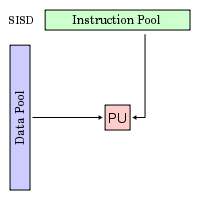
\includegraphics[width=0.50\textwidth]{parallel/SISD}
\caption{Single Instruction Single Data.}
\label{SISD}
\end{figure}

\subsection*{Single Instruction Multiple Data - SIMD}
Architectures based on SIMD uses  multiple processing units to execute a single instruction on multiple data. Thus SIMD uses data level parallelism as previously discussed. Modern CPUs are all able to perform SIMD instructions and they are able to load n numbers (n may vary depending on design) of data to memory at once and and execute the single instruction on the data. An example where SIMD instrctions can be used is in image preocessing where several pixels are to be added or subtracted the by samme value. How SIMD instructions works is shown in figure \ref{SIMD}
\begin{figure}[h!]
\centering
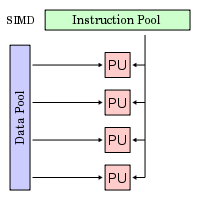
\includegraphics[width=0.50\textwidth]{parallel/SIMD}
\caption{Single Instruction Multiple Data.}
\label{SIMD}
\end{figure}
asd
\subsection*{Multiple Instruction Single Data - MISD}
MISD is the least used archetecture type of the four in Flynn's taxonomy. This is because doing multiple instructions on a single data is much less scalable and it does not utilize computational resources as good as the rest. MISD is illustrated in figure \ref{MISD}.
\begin{figure}[h!]
\centering
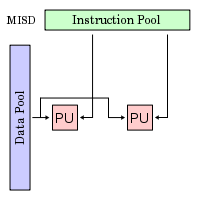
\includegraphics[width=0.50\textwidth]{parallel/MISD}
\caption{Multiple Instruction Single Data.}
\label{MISD}
\end{figure}

\subsection*{Multiple Instruction Multiple Data - MIMD}
Being able to do multiple instructions on multiple data is possible by having different processors execute instructions on multiple data. Modern CPUs consisting of several cores are all based on MIMD for parallelism. MIMD is illustrated in figure \ref{MIMD}.
\begin{figure}[h!]
\centering
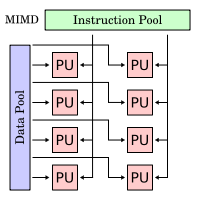
\includegraphics[width=0.50\textwidth]{parallel/MIMD}
\caption{Multiple Instruction Multiple Data.}
\label{MIMD}
\end{figure}

\section{Graphics processing unit}
A graphics processing unit (GPU) is a specialized chip that initially was designed to offload the CPU and accelerate processes associated with computer graphics. The process of computing the color of each pixel on screen is memory intensive but independent of each other and thus highly parallelizable. 

\section{OpenMP}
OpenMP is an API that supports shared memory parallel programming in C, C++, and Fortran for multiple processor architecture types and operative systems. TODO

\section{General Purpose GPU}
TODO 

\section{CUDA}
TODO
